\documentclass[aspectratio=169,11pt]{beamer}

% ---------- Theme ----------
\usetheme{Madrid}
\usecolortheme{default}
\setbeamertemplate{navigation symbols}{}
\setbeamertemplate{footline}[frame number]

% ---------- Shared preamble ----------
% preamble_common.tex — Shared packages and macros for report & slides
%
% Usage:
%   % preamble_common.tex — Shared packages and macros for report & slides
%
% Usage:
%   % preamble_common.tex — Shared packages and macros for report & slides
%
% Usage:
%   \input{preamble_common}   (after \documentclass)

% ---------- Packages ----------
\usepackage[utf8]{inputenc}
\usepackage[T1]{fontenc}
\usepackage{amsmath,amssymb}
\usepackage{graphicx}
\usepackage{booktabs}
\usepackage{siunitx}
\usepackage{hyperref}
\usepackage{cleveref}
\usepackage{tikz}
\usetikzlibrary{arrows.meta, positioning, calc, decorations.pathmorphing}

% ---------- SI unit setup ----------
\sisetup{
  per-mode=symbol,
  inter-unit-product=\ensuremath{\cdot},
  separate-uncertainty=true
}
\DeclareSIUnit{\um}{\micro\metre}

% ---------- Custom macros ----------
\newcommand{\kpole}{k_\mathrm{pole}}
\newcommand{\Ra}{R_\mathrm{a}}
\newcommand{\SH}{S_\mathrm{H}}
\newcommand{\kA}{k_\mathrm{A}}
\newcommand{\Nc}{N_\mathrm{c}}
\newcommand{\rtip}{r_\mathrm{tip}}
\newcommand{\Vda}{V_\mathrm{DA}}
\newcommand{\Vm}{V_\mathrm{m}}
\newcommand{\Fmag}{F_\mathrm{mag}}
\newcommand{\Fthermal}{F_\mathrm{thermal}}
\newcommand{\chitot}{\chi_\mathrm{eff}}
\newcommand{\Vbead}{V_\mathrm{bead}}
   (after \documentclass)

% ---------- Packages ----------
\usepackage[utf8]{inputenc}
\usepackage[T1]{fontenc}
\usepackage{amsmath,amssymb}
\usepackage{graphicx}
\usepackage{booktabs}
\usepackage{siunitx}
\usepackage{hyperref}
\usepackage{cleveref}
\usepackage{tikz}
\usetikzlibrary{arrows.meta, positioning, calc, decorations.pathmorphing}

% ---------- SI unit setup ----------
\sisetup{
  per-mode=symbol,
  inter-unit-product=\ensuremath{\cdot},
  separate-uncertainty=true
}
\DeclareSIUnit{\um}{\micro\metre}

% ---------- Custom macros ----------
\newcommand{\kpole}{k_\mathrm{pole}}
\newcommand{\Ra}{R_\mathrm{a}}
\newcommand{\SH}{S_\mathrm{H}}
\newcommand{\kA}{k_\mathrm{A}}
\newcommand{\Nc}{N_\mathrm{c}}
\newcommand{\rtip}{r_\mathrm{tip}}
\newcommand{\Vda}{V_\mathrm{DA}}
\newcommand{\Vm}{V_\mathrm{m}}
\newcommand{\Fmag}{F_\mathrm{mag}}
\newcommand{\Fthermal}{F_\mathrm{thermal}}
\newcommand{\chitot}{\chi_\mathrm{eff}}
\newcommand{\Vbead}{V_\mathrm{bead}}
   (after \documentclass)

% ---------- Packages ----------
\usepackage[utf8]{inputenc}
\usepackage[T1]{fontenc}
\usepackage{amsmath,amssymb}
\usepackage{graphicx}
\usepackage{booktabs}
\usepackage{siunitx}
\usepackage{hyperref}
\usepackage{cleveref}
\usepackage{tikz}
\usetikzlibrary{arrows.meta, positioning, calc, decorations.pathmorphing}

% ---------- SI unit setup ----------
\sisetup{
  per-mode=symbol,
  inter-unit-product=\ensuremath{\cdot},
  separate-uncertainty=true
}
\DeclareSIUnit{\um}{\micro\metre}

% ---------- Custom macros ----------
\newcommand{\kpole}{k_\mathrm{pole}}
\newcommand{\Ra}{R_\mathrm{a}}
\newcommand{\SH}{S_\mathrm{H}}
\newcommand{\kA}{k_\mathrm{A}}
\newcommand{\Nc}{N_\mathrm{c}}
\newcommand{\rtip}{r_\mathrm{tip}}
\newcommand{\Vda}{V_\mathrm{DA}}
\newcommand{\Vm}{V_\mathrm{m}}
\newcommand{\Fmag}{F_\mathrm{mag}}
\newcommand{\Fthermal}{F_\mathrm{thermal}}
\newcommand{\chitot}{\chi_\mathrm{eff}}
\newcommand{\Vbead}{V_\mathrm{bead}}


% ---------- Beamer-specific ----------
\usepackage{appendixnumberbeamer}

% ---------- Title info ----------
\title[Charge Calibration]{Magnetic Charge Calibration of a\\
Yokeless Hexapole Actuator}
\subtitle{Inverse-Square Law Fitting \& Physical Analysis}
\author{PME406 Laboratory}
\institute{Department of Mechanical Engineering\\
National Taiwan University}
\date{\today}

% ============================================================
\begin{document}

% ---- Slide 1: Title ----
\begin{frame}
\titlepage
\end{frame}

% ---- Slide 2: Motivation ----
\begin{frame}{Motivation}
\begin{itemize}
\item Hexapole electromagnetic actuators generate magnetic field gradients
      for micro/nanomanipulation
\item Key question: \textbf{How does the field decay with distance for a
      yokeless configuration?}
\item The \emph{magnetic charge offset} $b$ quantifies flux concentration:
\end{itemize}

\vspace{0.5em}
\begin{block}{Core Model}
\[
H(x) = \frac{a^2}{(x + b)^2}
\quad\Longrightarrow\quad
\frac{1}{\sqrt{H}} = \frac{x}{a} + \frac{b}{a}
\]
\end{block}

\vspace{0.5em}
\begin{itemize}
\item Smaller $b$ = tighter flux concentration = stronger forces
\item This work: determine $b$ for a yokeless hexapole and compare with
      Menq's yoke design ($b = \SI{405}{\um}$)
\end{itemize}
\end{frame}

% ---- Slide 3: Signal Chain ----
\begin{frame}{Signal Chain}
\centering
\begin{tikzpicture}[
    block/.style={draw, thick, minimum width=1.8cm, minimum height=0.8cm,
                  font=\small},
    arr/.style={-{Stealth[length=2.5mm]}, thick},
    lbl/.style={font=\scriptsize, midway, above}
]
\node[block] (dac) {DAC};
\node[block, right=1.0cm of dac] (amp) {Amp};
\node[block, right=1.0cm of amp] (coil) {Coil};
\node[block, right=1.0cm of coil] (mono) {Monopole};
\node[block, right=1.0cm of mono] (hall) {Hall};

\draw[arr] (dac) -- node[lbl] {$\Vda$} (amp);
\draw[arr] (amp) -- node[lbl] {$I$} (coil);
\draw[arr] (coil) -- node[lbl] {$\Phi$} (mono);
\draw[arr] (mono) -- node[lbl] {$B(x)$} (hall);
\draw[arr] (hall.east) -- ++(0.8,0) node[right, font=\small] {$\Vm$};

\node[font=\tiny, below=0.1cm of amp] {$\kA$};
\node[font=\tiny, below=0.1cm of coil] {$\Nc, \Ra$};
\node[font=\tiny, below=0.1cm of mono] {$q = \Phi/\mu_0$};
\node[font=\tiny, below=0.1cm of hall] {$\SH$};
\end{tikzpicture}

\vspace{1em}
\begin{columns}[T]
\column{0.5\textwidth}
\begin{block}{Known Constants}
\begin{itemize}\small
\item $\kA = \SI{0.3614}{\ampere/\volt}$
\item $\Nc = 50$ turns
\item $\SH = \SI{130}{\volt/\tesla}$
\end{itemize}
\end{block}
\column{0.5\textwidth}
\begin{block}{Key Result}
\[
H(x) = \frac{\SH \cdot \kpole \cdot \kA}{4\pi(x+b)^2} \times 10^{12}
\]
$\mu_0$ cancels in monopole model!
\end{block}
\end{columns}
\end{frame}

% ---- Slide 4: Monopole Model ----
\begin{frame}{Monopole Model}
\centering
\begin{tikzpicture}[>=Stealth, thick, scale=0.85, every node/.style={scale=0.85}]
\fill[gray!20] (-3.0,-.7) rectangle (-0.3,.7);
\draw[thick] (-3.0,-.7) rectangle (-0.3,.7);
\node at (-1.65, 0) {Pole};
\draw[thick] (-0.3, 0.4) .. controls (0.05, 0.4) and (0.15, 0.25) .. (0.15, 0)
             .. controls (0.15, -0.25) and (0.05, -0.4) .. (-0.3, -0.4);
\draw[dashed, gray] (0.15, -1.0) -- (0.15, 1.0);
\node[circle, fill=black, inner sep=1.5pt, label={below:\small$q$}] at (-0.8, 0) {};
\draw[{Stealth}-{Stealth}] (-0.8, -0.85) -- (0.15, -0.85);
\node[below, font=\small] at (-0.33, -0.85) {$b$};
\node[draw, thick, minimum width=0.5cm, minimum height=0.8cm,
      fill=blue!10] (sensor) at (3.0, 0) {};
\node[font=\tiny, below=0.05cm of sensor] {Hall};
\draw[{Stealth}-{Stealth}] (0.15, 0.85) -- (2.75, 0.85);
\node[above, font=\small] at (1.45, 0.85) {$x$};
\draw[-{Stealth}, blue] (0.4, 0) -- (2.6, 0);
\end{tikzpicture}

\vspace{0.5em}
\begin{columns}[T]
\column{0.5\textwidth}
\begin{block}{Field (Coulomb's law)}
\[
B(x) = \frac{\kpole \, I}{4\pi(x+b)^2}
\]
\end{block}
\column{0.5\textwidth}
\begin{block}{Force on bead}
\[
\Fmag = \frac{\chitot \Vbead}{\mu_0} B \left|\frac{dB}{dx}\right|
\propto \frac{1}{(x+b)^5}
\]
\end{block}
\end{columns}
\end{frame}

% ---- Slide 5: Linearization ----
\begin{frame}{Linearization Strategy}
\begin{block}{Model}
\[
H(x) = \frac{a^2}{(x+b)^2}
\]
\end{block}

\begin{block}{Linearize: take reciprocal square root}
\[
y = \frac{1}{\sqrt{H(x)}} = \frac{x+b}{a} = \underbrace{\frac{1}{a}}_{\text{slope}} \cdot x + \underbrace{\frac{b}{a}}_{\text{intercept}}
\]
\end{block}

\vspace{0.5em}
\begin{itemize}
\item Ordinary least-squares regression on $y$ vs $x$
\item Recover: $a = 1/\text{slope}$, \quad $b = \text{intercept}/\text{slope}$
\item $R^2$ computed in linearized space
\item No iterative optimization needed --- closed-form solution
\end{itemize}
\end{frame}

% ---- Slide 6: Experiment Design ----
\begin{frame}{Experiment Design}
\begin{columns}[T]
\column{0.55\textwidth}
\begin{block}{Measurement Grid}
\begin{itemize}\small
\item \textbf{22 distances}: 10--\SI{2000}{\um}
\item \textbf{15 frequencies}: 0.1--\SI{3000}{\hertz}
\item \textbf{330 measurements}: 100\% valid
\end{itemize}
\end{block}

\vspace{0.5em}
\begin{block}{Hardware}
\begin{itemize}\small
\item Yokeless hexapole, $\rtip = \SI{5}{\um}$
\item EQ-730L Hall sensor ($\SH = 130$ V/T)
\item 16-bit DAC, $f_s = \SI{20}{\kilo\hertz}$
\end{itemize}
\end{block}

\column{0.45\textwidth}
\begin{block}{Processing Pipeline}
\begin{enumerate}\small
\item Steady-state detection (0.2\% threshold)
\item Super-period truncation (no spectral leakage)
\item FFT $\to$ $|H| = |V_m| / |V_{DA}|$
\item Linearize + fit
\end{enumerate}
\end{block}
\end{columns}
\end{frame}

% ---- Slide 7: Data Quality ----
\begin{frame}{Data Quality: Lissajous Figures (0.1 Hz)}
\centering
\includegraphics[height=0.75\textheight]{../results/Charge_NTU/figures/Charge_Lissajous_0p1Hz.png}%
\hfill
\includegraphics[height=0.75\textheight]{../results/Charge_NTU/figures/Charge_Lissajous_0p1Hz_Normalized.png}

\vspace{0.3em}
\small Elliptical traces confirm linear system behavior at all 22 distances.
\end{frame}

% ---- Slide 8: Raw Data ----
\begin{frame}{Raw Data: $|H(x)|$ at 0.1 Hz}
\centering
\includegraphics[height=0.8\textheight]{../results/Charge_NTU/figures/Charge_Fit_Single_0p1Hz.png}

\vspace{0.3em}
\small Dynamic range $\approx$ 4:1 over 10--\SI{2000}{\um}.
\end{frame}

% ---- Slide 9: Multi-Frequency Consistency ----
\begin{frame}{Multi-Frequency Overlay: 0.1, 1, 10 Hz}
\centering
\includegraphics[height=0.8\textheight]{../results/Charge_NTU/figures/Charge_Fit_Overlay.png}

\vspace{0.3em}
\small Three curves virtually indistinguishable --- $b$ is frequency-independent.
\end{frame}

% ---- Slide 10: Fitting Quality ----
\begin{frame}{Fitting Quality: $b$ and $R^2$ Consistency}
\centering
\includegraphics[height=0.8\textheight]{../results/Charge_NTU/figures/Charge_Fit_Summary.png}
\end{frame}

% ---- Slide 11: Linearized Fit ----
\begin{frame}{Linearized Fit: $1/\sqrt{H}$ vs Distance}
\centering
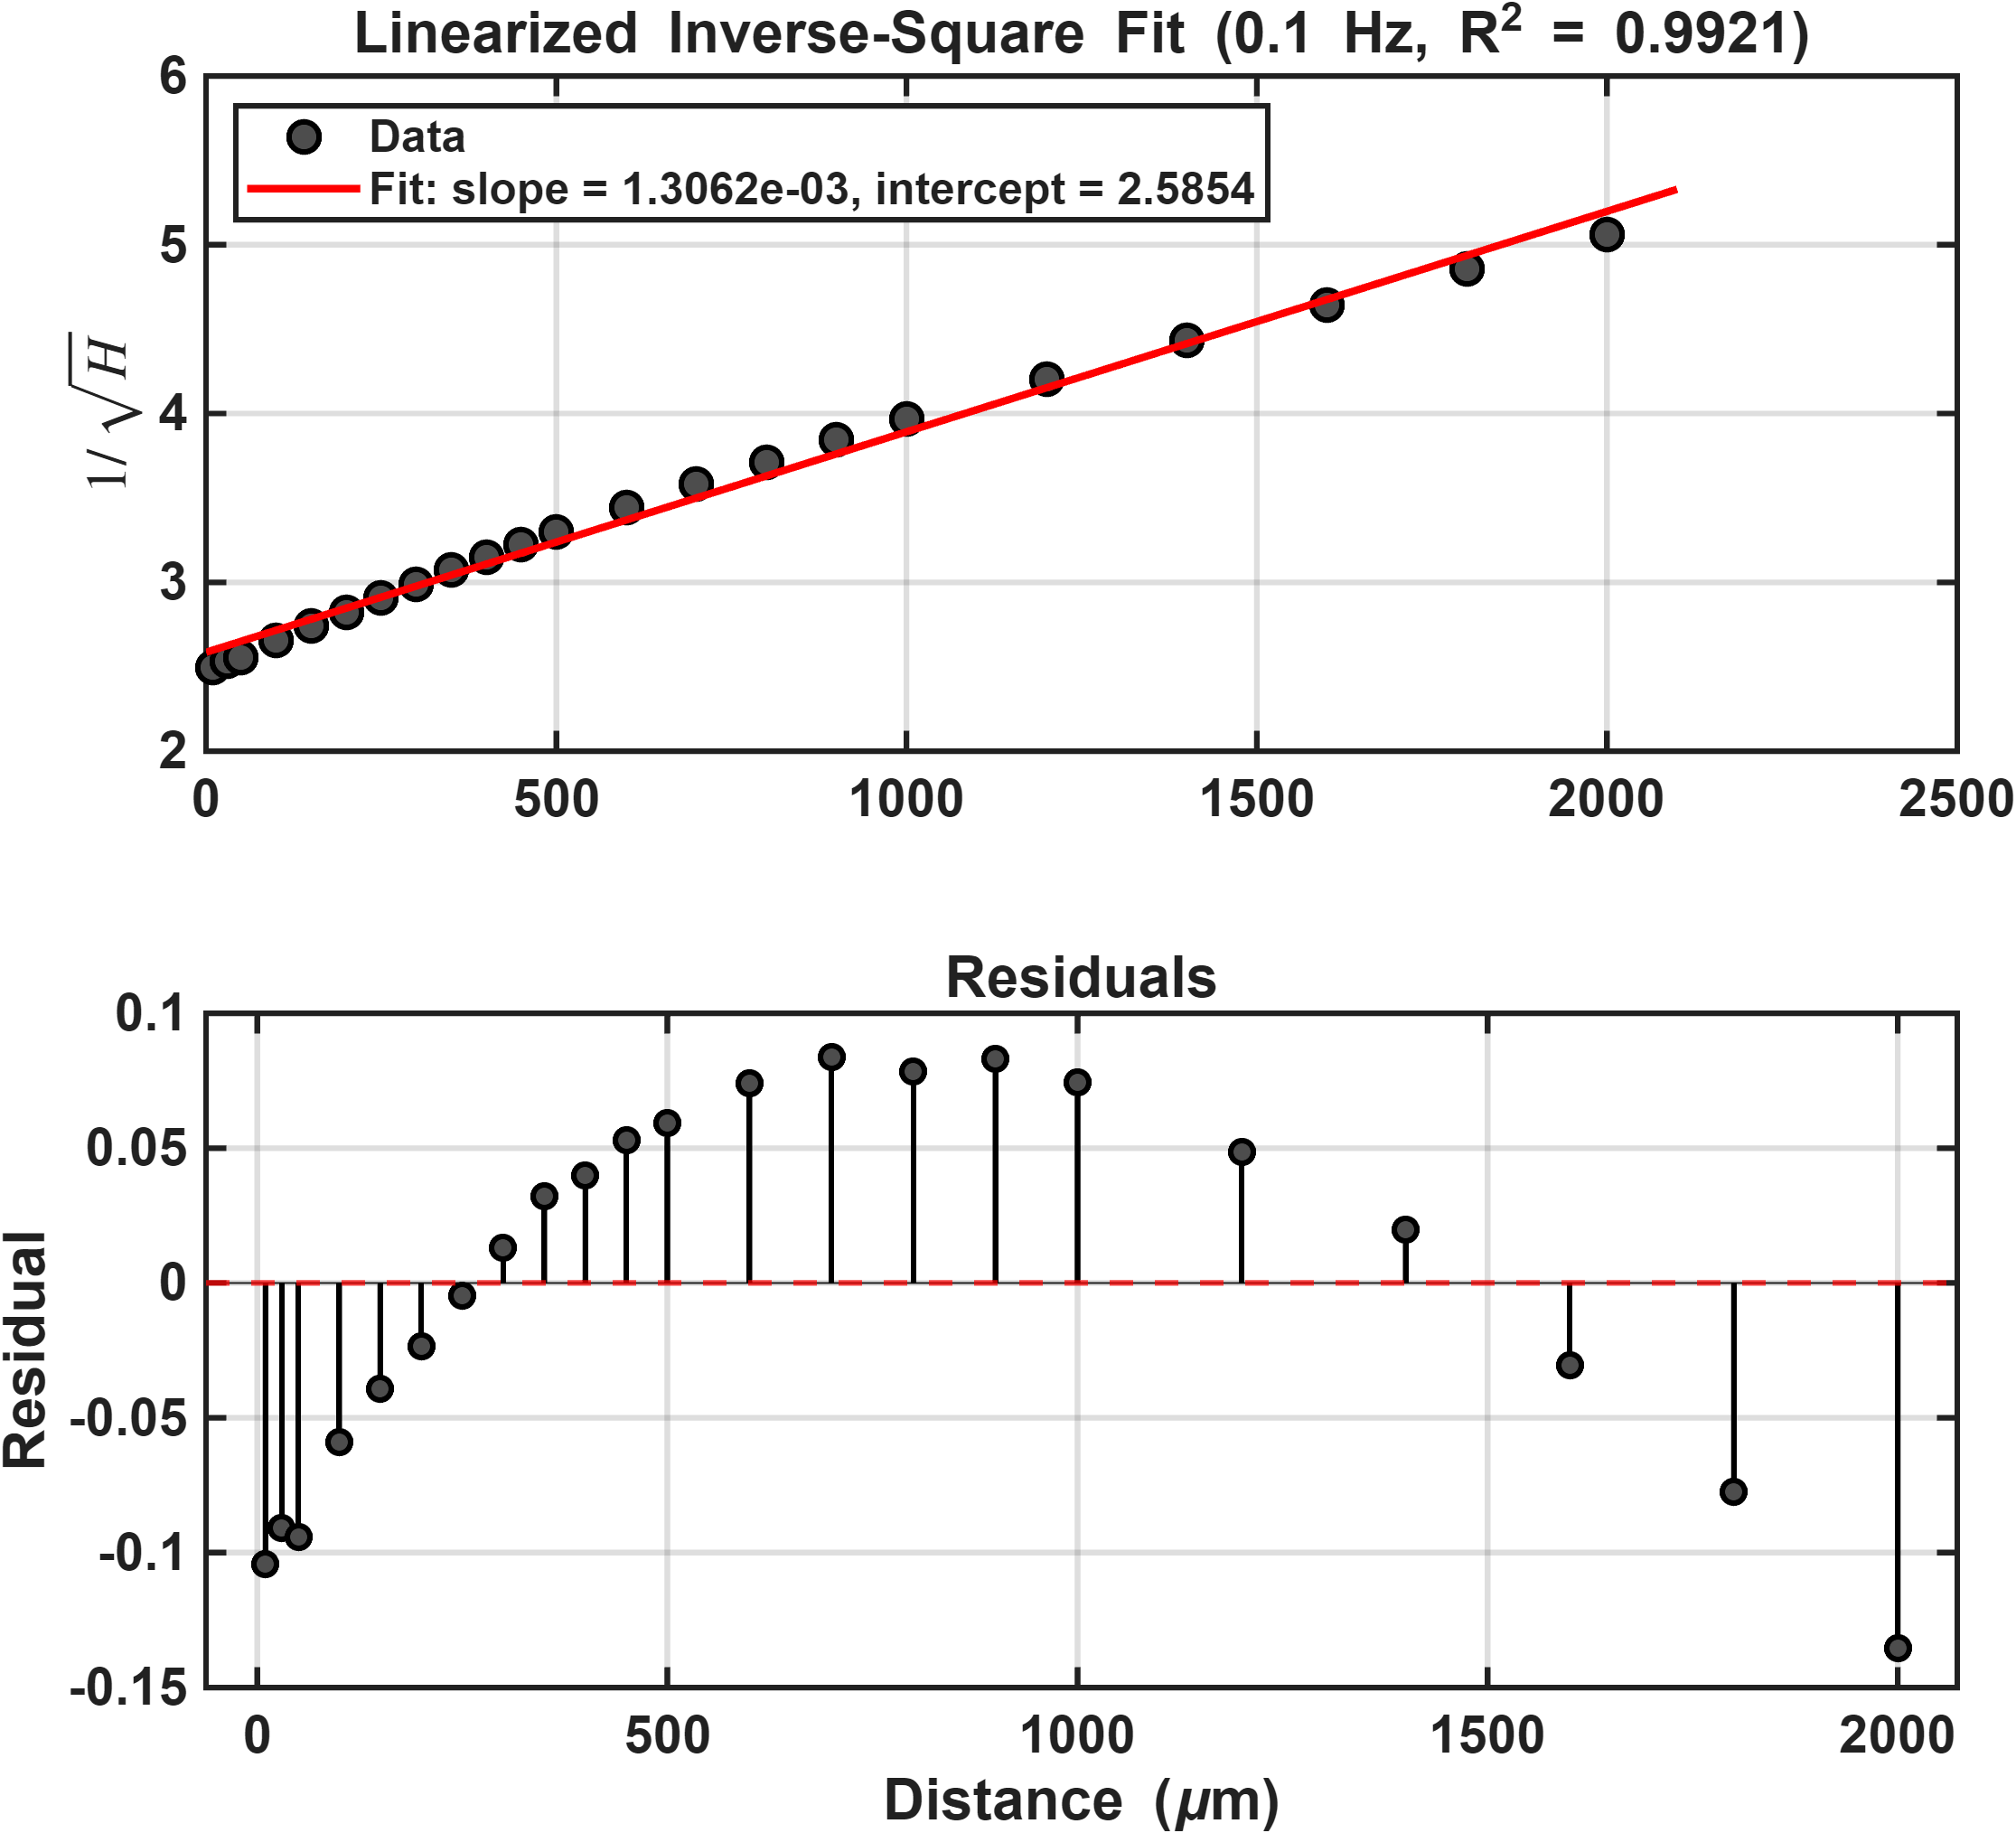
\includegraphics[height=0.8\textheight]{figures/linearized_fit.png}

\vspace{0.3em}
\small Perfect linearity confirms inverse-square law. Residuals show no trend.
\end{frame}

% ---- Slide 12: Distance Range Effect ----
\begin{frame}{Distance Range Effect on $b$}
\begin{columns}[T]
\column{0.55\textwidth}
\centering
\includegraphics[width=\textwidth]{../results/Charge_NTU/figures/Charge_Fit_Single_0p1Hz_10to500um.png}

\column{0.45\textwidth}
\vspace{1em}
\begin{block}{Range Dependence}
\begin{itemize}\small
\item Full range (10--2000 \si{\um}):\\$b = \SI{1979}{\um}$
\item Short range (10--500 \si{\um}):\\$b \approx \SI{1504}{\um}$
\end{itemize}
\end{block}

\vspace{0.5em}
\small \textbf{Why?} At short distances, multipole corrections bias $b$
downward. Full-range estimate captures the true monopole component.
\end{columns}
\end{frame}

% ---- Slide 13: Physical Parameters ----
\begin{frame}{Derived Physical Parameters}
\begin{block}{From fitted $a = 765.35$:}
\begin{align*}
\kpole &= \frac{4\pi \, a^2}{\SH \cdot \kA \times 10^{12}}
        = 1.57 \times 10^{-7} \;\text{Wb/A} \\
\Ra    &= \frac{\Nc}{\kpole}
        = 3.19 \times 10^{8} \;\text{A/Wb} \quad (\text{total, no yoke})
\end{align*}
\end{block}

\vspace{0.3em}
\centering
\small
\begin{tabular}{lccc}
\toprule
Parameter & This work & Menq 2010 & Menq 2011 \\
\midrule
Config   & Hexapole (no yoke) & Quad (yoke) & Hex (yoke) \\
$\Nc$    & 50     & 200    & 200 \\
$\rtip$ (\si{\um}) & 5 & 40 & 40 \\
$\kpole$ (Wb/A) & $1.57 \times 10^{-7}$ & --- & --- \\
$b$ (\si{\um}) & \textbf{1979} & \textbf{405} & --- \\
\bottomrule
\end{tabular}

\vspace{0.5em}
\alert{$\Ra$ values are NOT comparable} (different definitions).
$b$ is the meaningful metric.
\end{frame}

% ---- Slide 14: Force Analysis ----
\begin{frame}{Force Analysis}
\centering
\includegraphics[height=0.8\textheight]{../results/Charge_NTU/figures/Charge_Physics_Analysis.png}
\end{frame}

% ---- Slide 15: Yoke Comparison ----
\begin{frame}{Yokeless vs Yoke: Field Decay Comparison}
\begin{columns}[T]
\column{0.55\textwidth}
\centering
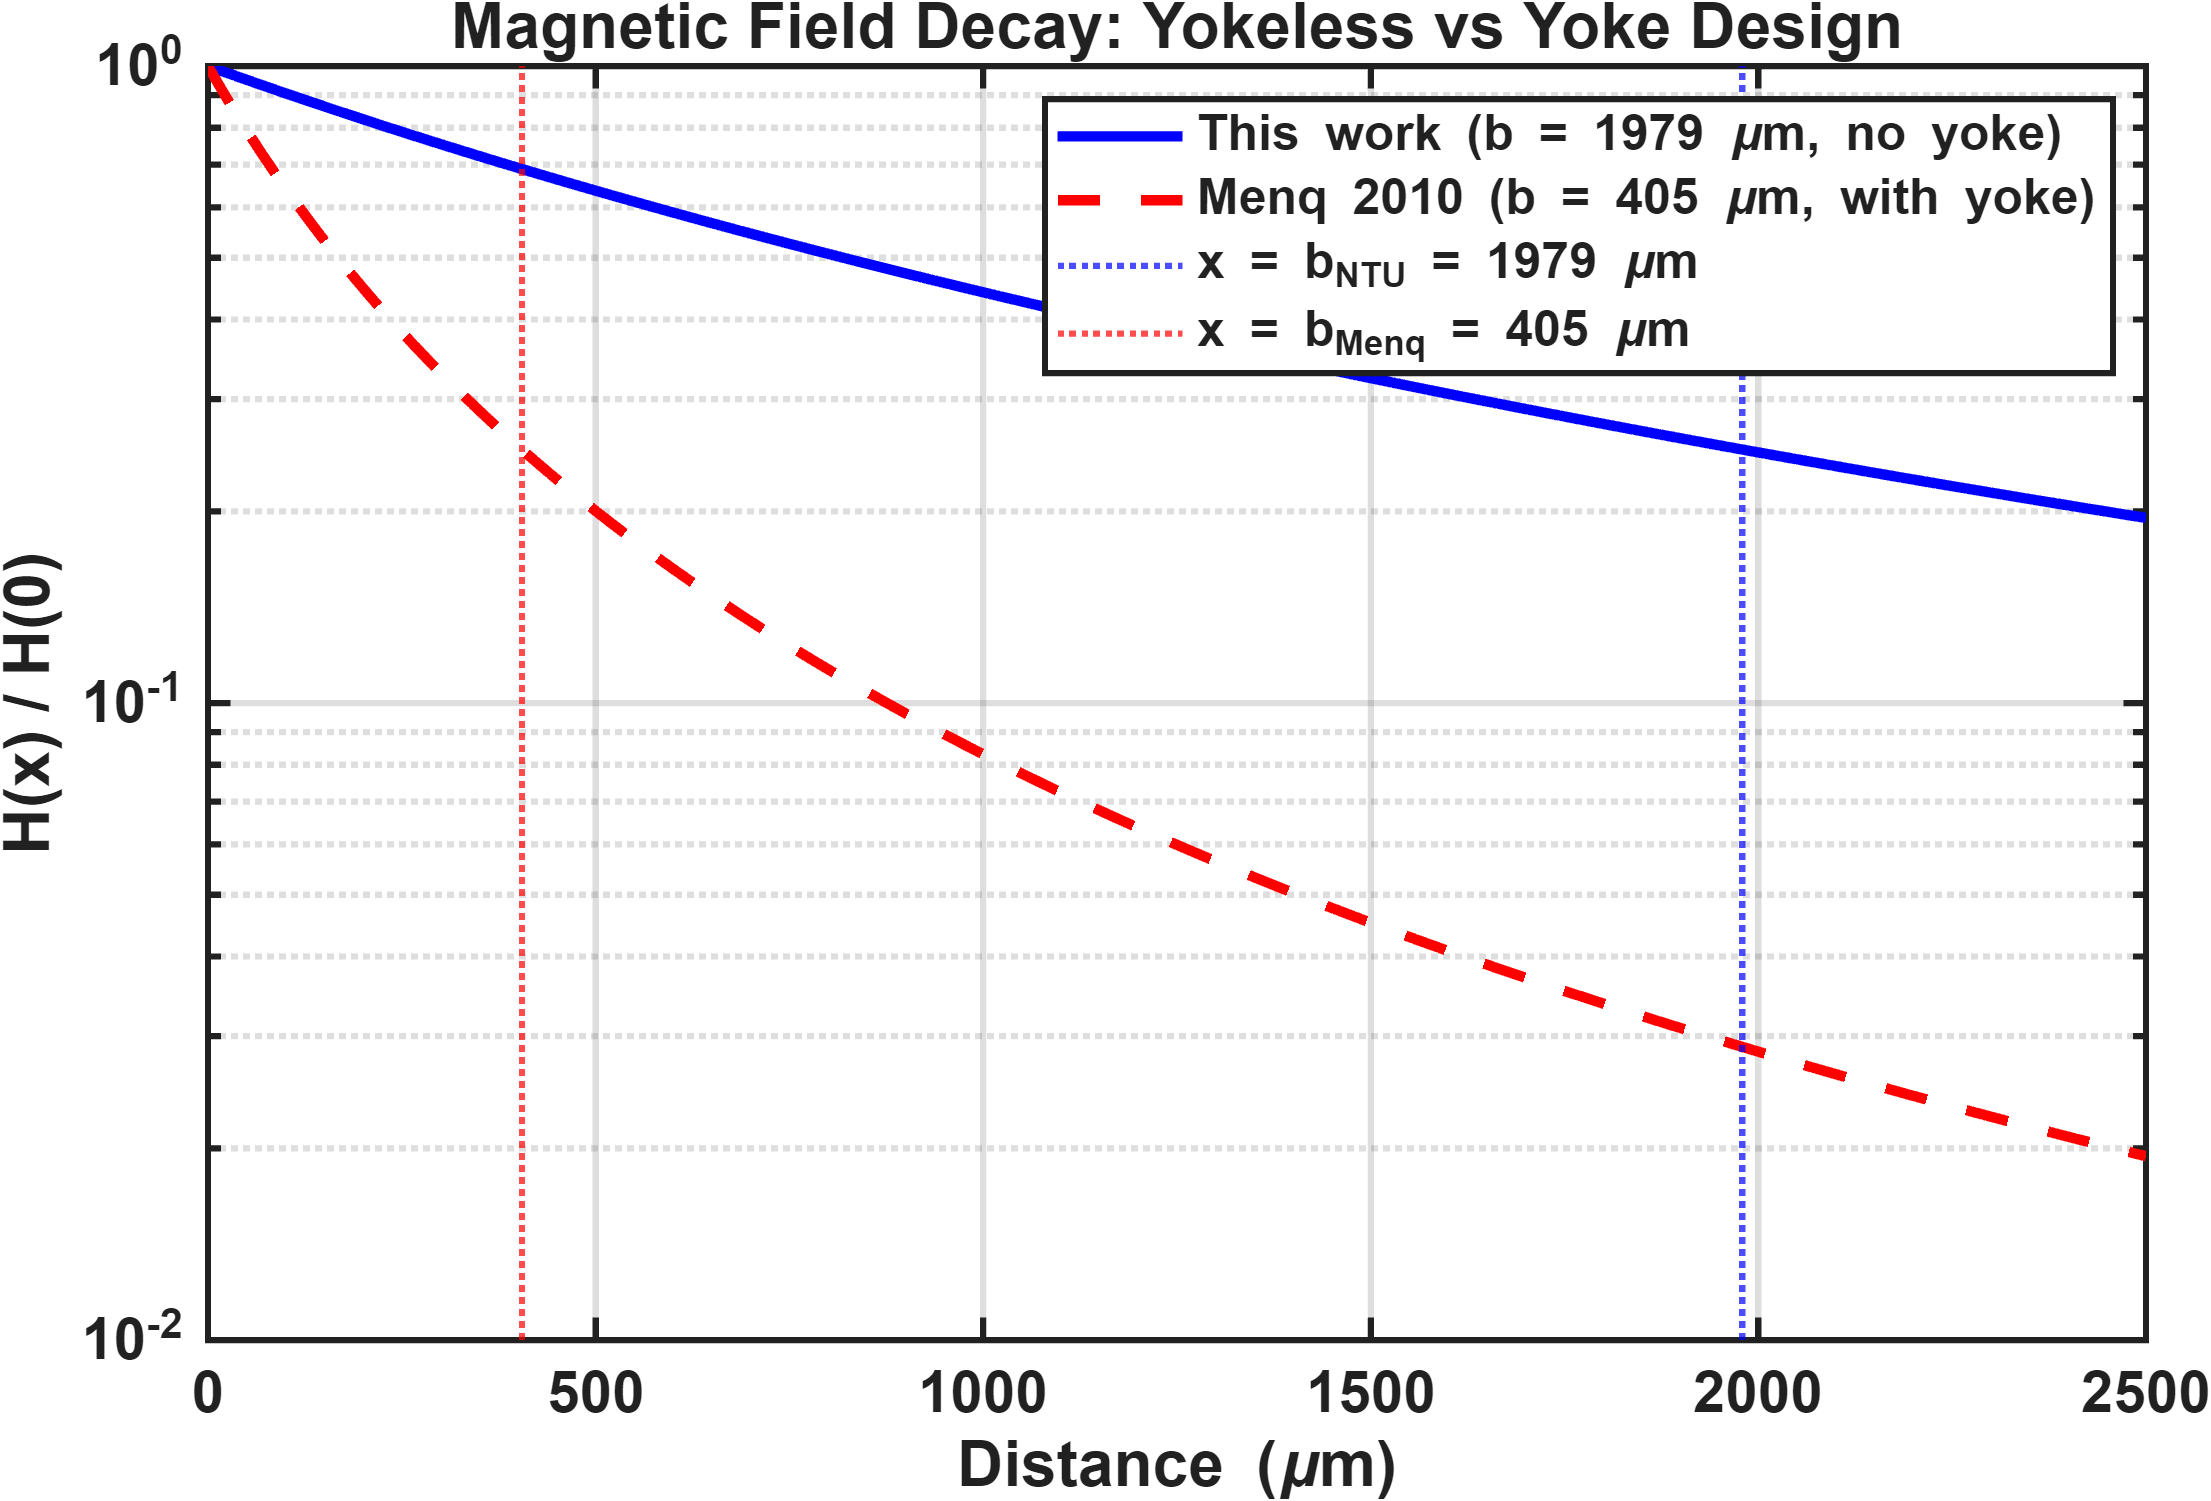
\includegraphics[width=\textwidth]{figures/yoke_comparison.png}

\column{0.45\textwidth}
\vspace{0.5em}
\begin{block}{Force Suppression}
\[
\frac{F_\text{real}}{F_\text{ideal}} = \left(\frac{\rtip}{\rtip + b}\right)^5
\approx 10^{-14}
\]
\end{block}

\vspace{0.5em}
\begin{itemize}\small
\item $b_\text{NTU} = \SI{1979}{\um}$ (no yoke)
\item $b_\text{Menq} = \SI{405}{\um}$ (yoke)
\item Yokeless: $\sim 240\times$ weaker force
\item Yoke provides low-$R$ return path $\to$ smaller $b$
\end{itemize}
\end{columns}
\end{frame}

% ---- Slide 16: Key Takeaways ----
\begin{frame}{Key Takeaways}
\begin{enumerate}
\item \textbf{Monopole model works.}\\
$H(x) = a^2/(x+b)^2$ fits with $R^2 > 0.991$;
$b = 1979 \pm \SI{1}{\um}$, frequency-independent.

\vspace{0.8em}
\item \textbf{Yoke is essential.}\\
Without yoke: $b = \SI{1979}{\um} \gg \rtip = \SI{5}{\um}$ $\to$
flux not concentrated $\to$ sub-pN forces.\\
With yoke (Menq): $b = \SI{405}{\um}$ $\to$ $\sim 240\times$ stronger.

\vspace{0.8em}
\item \textbf{$b$ is the figure of merit.}\\
Unlike $\Ra$ (topology-dependent definition), $b$ directly compares
flux concentration across any actuator geometry.
\end{enumerate}
\end{frame}

% ---- Slide 17: Next Steps ----
\begin{frame}{Next Steps}
\begin{itemize}
\item \textbf{Multi-pole characterization:} Repeat charge calibration for
all 6 poles $\to$ $b$ uniformity, inter-pole coupling

\vspace{0.5em}
\item \textbf{Yoke integration:} Add ferromagnetic yoke and re-measure $b$
to quantify improvement

\vspace{0.5em}
\item \textbf{Multipole model:} Fit monopole-plus-dipole to explain the
distance-range dependence of $b$

\vspace{0.5em}
\item \textbf{Force validation:} Direct force measurement on trapped bead
vs.\ model prediction
\end{itemize}
\end{frame}

% ---- Slide 18: Backup ----
\appendix
\begin{frame}{Backup: Representative Data}
\centering
\small
\begin{tabular}{r|ccc|cc}
\toprule
$x$ (\si{\um}) & $|H|_{0.1}$ & $|H|_{1}$ & $|H|_{10}$ & $|H|_{1000}$ & $|H|_{2000}$ \\
\midrule
10   & 0.1607 & 0.1601 & 0.1610 & 0.1378 & 0.1169 \\
100  & 0.1417 & 0.1422 & 0.1421 & 0.1216 & 0.1040 \\
500  & 0.0919 & 0.0920 & 0.0919 & 0.0788 & 0.0671 \\
1000 & 0.0636 & 0.0635 & 0.0635 & 0.0545 & 0.0462 \\
2000 & 0.0390 & 0.0391 & 0.0391 & 0.0337 & 0.0285 \\
\bottomrule
\end{tabular}

\vspace{1em}
\begin{tabular}{lcc}
\toprule
Freq (Hz) & $a$ & $b$ (\si{\um}) \\
\midrule
0.1 & 765.57 & 1979.3 \\
1   & 764.84 & 1977.6 \\
10  & 765.63 & 1979.9 \\
\midrule
Mean & $765.35 \pm 0.43$ & $1978.9 \pm 1.2$ \\
\bottomrule
\end{tabular}
\end{frame}

\end{document}
